\section{Cours 3}
\subsection{Dualité dans la programmation linéaire}
maximiser 2x$_1$+3x$_2$ avec:
\begin{itemize}
	\item 4x$_1$+8x$_2\leq$12
	\item 2x$_1$+x$_2\leq$3
	\item 3x$_1$+2x$_2\leq$4
	\item x$_1$,x$_2\geq$0
\end{itemize}
L'objectif est de calculer les bornes supérieures pour l'optimum sans résoudre le programme linéaire.
\begin{enumerate}
	\item Notons que 2x$_1$+3x$_2\leq$4x$_1$+8x$_2\leq$12$\Rightarrow$OPT$\leq$12
	\item Notons aussi 2x$_1$+3x$_2\leq\frac{1}{2}$(4x$_1$+8x$_2$)$\leq$6$\Rightarrow$OPT$\leq$6
	\item Aussi 2x$_1$+3x$_2$=$\frac{1}{3}$(4x$_1$+8x$_2$)+$\frac{1}{3}$(2x$_1$+x$_2$)$\leq\frac{12}{3}$+
	$\frac{3}{3}$=5$\Rightarrow$OPT$\leq$5
\end{enumerate}

\textbf{Cas général:}
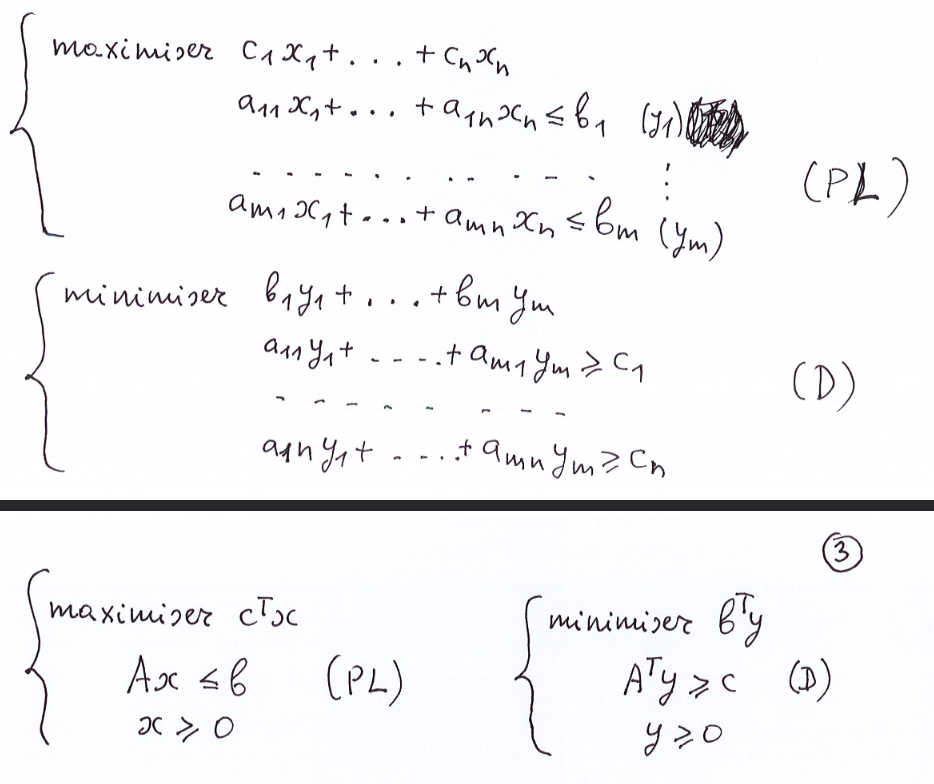
\includegraphics[width=\linewidth,height=0.75\textheight]{notes/algorithme/cas_general_dualite.png}
